%!TEX root = exam.tex
\begin{center}
    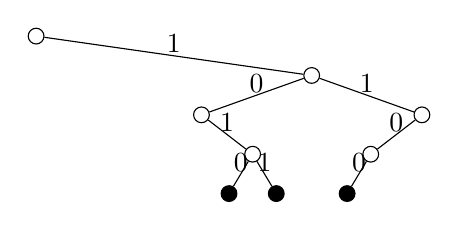
\begin{tikzpicture}[level distance=0.5cm,
        level 1/.style={sibling distance=7cm},
        level 2/.style={sibling distance=2.8cm},
        level 3/.style={sibling distance=1.3cm},
        level 4/.style={sibling distance=0.6cm},
        level 5/.style={sibling distance=0.2cm},
        every node/.style={draw,circle,inner sep=0pt,minimum size=2mm}]
        \node {}
        child[missing]
        child {
            node {}
            child {
                node {}
                child[missing]
                child {
                    node {}
                    child {
                        node[circle,draw,fill=black]{}
                        edge from parent node[draw=none,above] {0}
                    }
                    child {
                        node[circle,draw,fill=black]{}
                        edge from parent node[draw=none,above] {1}
                    }
                    edge from parent node[draw=none,above] {1}
                }
                edge from parent node[draw=none,above] {0}
            }            
            child {
                node {}
                child {
                    node {}
                    child {
                        node[circle,draw,fill=black]{}
                        edge from parent node[draw=none,above] {0}
                    }
                    child[missing]
                    edge from parent node[draw=none,above] {0}
                }
                child[missing]
                edge from parent node[draw=none,above] {1}
            }
            edge from parent node[draw=none,above] {1}
        }
        ;
    \end{tikzpicture}
\end{center}